\documentclass[a4paper, 12pt]{article}
\usepackage[top=8mm, bottom=8mm, left=18mm, right=18mm,
            headsep=6mm,
            headheight=40pt,
            includeheadfoot,
            bindingoffset=0mm]{geometry}
\renewcommand{\baselinestretch}{1.2}

\usepackage{hyperref}
\usepackage{tikz}

% ---CUSTOMISE ENUMERATION--- %
\usepackage{enumitem}

% ---FOR LANDSCAPE ORIENTED PAGES--- %
% \usepackage{lscape}

% ---ABSOLUTE TEXT POSITIONS--- %
\usepackage[absolute,overlay]{textpos}

% ---USE DIFFERENT FONTS--- %
% Uncomment the following 2 lines if you wanna use tetex and ...
%\usepackage{fontspec}
%\newfontfamily\headerfont{TeX Gyre Heros Bold}
% ... comment out this definition command "headerfont" which says to do nothing:
\newcommand{\headerfont}{}

% ---MATH AND EQUATION PACKAGES--- %
% \usepackage{amsmath, amssymb}
% \DeclareMathOperator{\sign}{sgn}
% \newcommand*\diff{\mathop{}\!\mathrm{d}}
% \usepackage{siunitx}

% ---SHADED TEXT AND TEXT COLOR--- %
% \usepackage{framed}
 \usepackage{xcolor}
 \definecolor{iwtdark}{HTML}{9d3238}
 \definecolor{iwtlight}{HTML}{cd8d25}
 \colorlet{shadecolor}{iwtlight!25}

% ---CHANGE PAGE HEADERS--- %
\usepackage{fancyhdr}
\usepackage{xpatch}
\xpretocmd\headrule{\color{lightgray}}{}{\PatchFailed}
\renewcommand{\headrulewidth}{0.6mm}% 2pt header rule
\fancyhf{} % sets both header and footer to nothing
\fancyhead[L]{
    \headerfont\scriptsize
    \textcolor{iwtdark}{
      Data Management Guidelines: \\
      How To Handle Data
    }
    \vfill
}
\fancyhead[R]{
 
\includegraphics[height=12mm]{Figure00_IWT-Logo.png}
}
\fancyfoot[C]{\headerfont\fontseries{bx}\textcolor{iwtdark}{\thepage}}
\fancypagestyle{plain}{
   \fancyhf{} % sets both header and footer to nothing
   \fancyfoot[CO, CE]{\headerfont\fontseries{bx}\textcolor{iwtdark}{\thepage}}
}
\pagestyle{fancy}

% ---CHANGE HEADING LAYOUT--- %
\usepackage{titlesec}
\titleformat{\section}[hang]%
  {\normalfont\fontseries{bx}}%
  {\headerfont\Large\fontseries{bx}\color{iwtdark}\thesection}%
  {1em}{\headerfont\fontseries{bx}\Large\color{iwtdark}}

\titleformat{\subsection}[hang]%
  {\normalfont\fontseries{bx}}%
  {\headerfont\large\fontseries{bx}\color{iwtdark}\thesubsection}%
  {1em}{\headerfont\fontseries{bx}\large\color{iwtdark}}

\titleformat{\subsubsection}[hang]%
  {\normalfont\fontseries{bx}}%
  {\headerfont\fontseries{bx}\color{iwtdark}\thesubsubsection}%
  {1em}{\headerfont\fontseries{bx}\color{iwtdark}}

\titleformat{\paragraph}[hang]%
  {\normalfont\normalsize\bfseries}%
  {\theparagraph}%
  {1em}{\headerfont\normalsize\bfseries\color{iwtdark}}

% ---INCLUDE FIGURES--- %
\usepackage{graphicx}
\graphicspath{{../../02_Figures/}}
\usepackage[font=small,labelfont=bf,justification=justified,
            singlelinecheck=false]{caption}
\usepackage{subcaption}
\usepackage{wrapfig}

% ---CHANGE TABLE LAYOUT--- %
\usepackage{booktabs}
\usepackage{makecell}
\usepackage{tabularx}
\usepackage{multirow}

% ---AUTOMATED BIBLIOGRAPHY--- %
\usepackage{biblatex}
\addbibresource{../../06_References/references.bib}
\usepackage{csquotes}

% ---INCLUDE PDFS--- %
% \usepackage{pdfpages}

% ---PSEUDOCODE --- %
% \usepackage{algorithm}
% \usepackage[noend]{algpseudocode}
% \makeatletter
% \def\BState{\State\hskip-\ALG@thistlm}
% \makeatother

\usepackage[ngerman]{babel}

% ---CUSTOM COMMANDS--- %
\newcommand{\tabitem}{~~\llap{\textbullet}~~}
\newcommand{\documenttitle}{Data Management Guidelines:\\ Wie man mit Daten umgeht}

\newcommand{\documentauthor}{Norbert Riefler}

\title{\documenttitle}
\begin{document}

\begin{titlepage}
  %\includepdf[pages=-]{figures/Titlepage.pdf}
  \tikz[remember picture,overlay] \node[opacity=0.7,inner sep=0pt] at (current page.center){
\includegraphics[width=1.05\paperwidth,height=1.05\paperheight]{Figure01_Titlepage_Background.pdf}};
  \begin{textblock*}{10cm}(1.5cm,16cm) % {block width} (xcoord, ycoord)
    \noindent
    \raggedright
    \textcolor{white}{
      \Huge\headerfont\fontseries{m}\documenttitle \\
      \vspace{6cm}
      \large\today
    }
  \end{textblock*}
  \begin{textblock*}{5cm}(15.4cm,28.5cm)
    \noindent
    \raggedright
    \textcolor{white}{
      \large\headerfont\fontseries{bx}\documentauthor
    }
  \end{textblock*}
\end{titlepage}
\newpage
\thispagestyle{empty}
\begin{center}
  \large\headerfont\fontseries{m}\textcolor{iwtdark}{Preface}
\end{center}

\begin{quote}
  `On July 20, 1969, Neil Armstrong climbed out of his spacecraft and
  placed his feet on the moon. The landing was broadcast live all over the
  world and was a significant event in both scientific and human History.
  Today, we can still watch the grainy video of the moon landing but what we
  cannot do is watch the original, higher quality footage or examine some of
  the data from this mission. This is because much of the data from early space
  exploration is lost forever. (...) The tapes were likely wiped and reused for
  data storage sometime in the 1970s.' \\
  \null\hfill - \citeauthor{briney2015}\cite{briney2015}
\end{quote}

\noindent This reader (https://github.com/Leibniz-IWT/DataManagementGuidelines) holds for all employees of the Leibniz-Institute for Materials Engineering (IWT) and serves as a reference
for how to save data. It delivers reasons for the question of why one should
think about data management and gives instructions and examples. Data management
in the information age is an absolutely required skill and a base to cope with
the wealth of data to avoid an information overload. It helps organizing
everyone’s own data, but it is also mandatory for data sharing so that others
can understand the structure and are able to interpret the information given by
your data. In this way, your data meet the FAIR standard (Findable, Accessible,
Interoperable and Reusable), basis for the looming new discipline of data science.

There are many topics in data management like data governance and security or
storage management, but we are treating here only a condensed extract, tailored
to data handling in our department. Therefore, this reader might help you to
clarify what must be done to be a data steward.
\newpage

\tableofcontents
% \listoffigures
% \listoftables
\newpage
\section{Why Data Management}

\textbf{Save time} \\
Planning your data management needs will save you time and resources, e.g.,
by faster locating data. And well managed data requires less preparation for
sharing or writing a paper. \\[6pt]
\textbf{Preserve your data} \\
Depositing your data in a file server (repository) safeguards your investment
of time and resources while preserving your research contribution for you and
others to use. \\[6pt]
\textbf{Increase your research impact} \\
Making your data available to other researchers can impact discovery and
relevance of your research. \\[6pt]
\textbf{Maintain data integrity} \\
Managing and documenting your data throughout its life cycle will allow you
and others to understand and use your data in the future. \\[6pt]
\textbf{Meet grant requirements} \\
Many funding bodies now require that researchers deposit data collected as
part of a research project. \\[6pt]
\textbf{Promote new discoveries} \\
Sharing your data with other researchers can lead to new and unanticipated
discoveries and provide research material for those with little or no funding. \\[6pt]
\textbf{Support open access} \\
Be a catalyst for research and discovery. Show your support for open access
by sharing your data.

\section{Pläne zur Datenverwaltung}

Der Umgang mit den Daten im Rahmen eines Projekts beinhaltet verschiedene
Aspekte, die in einem Datenmanagementplan (DMP) beschrieben werden. Ein DMP
enthält strukturierte Informationen über den Forschungsprozess des jeweiligen
Projekts. Diese Informationen müssen jedoch vor Projektbeginn vorliegen:
Antragsteller müssen in jedem Antrag einen DMP erstellen, der von allen
wichtigen Forschungsförderorganisationen (DFG, BMBF, etc.) gefordert wird.
Die Antragstellenden machen sich also schon beim Schreiben des Antrags Gedanken
darüber, wie sie mit den Daten umgehen wollen. Die folgenden Themen gehören zu
den typischen DMPs und könnten für Sie von Interesse sein:
\begin{enumerate}
  \item Administrative Informationen: Projektname, Art der Finanzierung, Zeitraum.
  \item Methoden der Datenerzeugung: Simulationen, Experimente (Geräte),
        Datenumfang, Art der Datendokumentation.
  \item Datensicherheit: Speicherort, Speicherintervall und -kapazität,
        wer hat Zugriff.
  \item Archivierung: welche Daten werden wo mit welchen Metadaten versehen.
  \item Gemeinsame Nutzung von Daten: welches Repository, Lizenzbedingung,
        welche erforderlichen Metadaten
  \item Ressourcen und Zuständigkeit: wer ist zuständig für Prozesse, IT,
        Festlegung von Vorgaben und Formaten, Überwachung; erforderliche
        personelle Ressourcen; Kosten.
\end{enumerate}
Weitere Einzelheiten finden Sie in \cite{dfg2021,hannover2020} sowie im Anhang; einige beispielhafte DMP sind auch hier zu finden: \\
\url{https://www.cms.hu-berlin.de/de/dl/dataman/arbeiten/dmp_erstellen}

\section{File Organization}
The following explains what and how to save your files on our servers:
\begin{itemize}
  \item Access to the VT-Server is established with your Web browser by typing
        \textbf{\url{http://134.102.40.154}} or
        \textbf{\url{http://vt-nas.mvt-bremen.de}}
        in the address field, via mapping the VT-Server to the Windows Explorer
        as an own drive, or by using the Synology Drive Client
        (see \cite{synology2022}) with some more and very helpful options like,
        e.g., document versioning. The \textbf{maximum size} of uploaded data
        should not exceed \textbf{100Gbyte per file}. Access privilege is
        administrated by
        Stefan Endres (\href{mailto:s.endres@iwt.uni-bremen.de}%
                       {s.endres@iwt.uni-bremen.de}),
        Arvind Chouhan (\href{mailto:a.chouhan@iwt.uni-bremen.de}%
                        {a.chouhan@iwt.uni-bremen.de})
        and Nils Ellendt (\href{mailto:ellendt@iwt.uni-bremen.de}%
                          {ellendt@iwt.uni-bremen.de}).
  \item The server of the manufacturing technology (FT) division is accessed via
        \textbf{\textbackslash\textbackslash fts-ags.iwt.uni-bremen.de}
        or \textbf{\textbackslash\textbackslash fts-ags}
        or \textbf{\textbackslash\textbackslash 134.102.244.1} in the
        windows explorer. Access privilege is administrated by the IWT IT
        division.
\end{itemize}

\subsection{Different Data Types}
Depending on the origin of the data, we distinguish between two data types:
\begin{itemize}
  \item Primary data (sometimes called raw data) is generated by measurement
        devices, sensors/cameras, simulation programs, observations etc. and
        are untreated; it is collected for the first time by the researcher.
  \item Secondary (or analyzed) data are processed primary data. (In social
        science, secondary data are already collected or produced data by
        others).
\end{itemize}
Very large primary data cannot be saved on our ELN%
\footnote{The use of the Electronic Lab Notebook (ELN) is currently only
mandatory for the VT. },
but the origin of that data are discussed there together with information about
the storage location (e.g. somewhere on a file server). The decision about the
limit, which data is considered as large, is:
\begin{itemize}
  \item data < 100 MByte is stored and documented on the ELN
  \item 100 MByte  < data < 1TByte is stored on the VT-Server and documented
        on the ELN
  \item data > 1 TByte is stored on USB-Disks and documented on the ELN
\end{itemize}
It is absolutely required that \textbf{all data from external sources} (e.g. by an USB
stick) have to be checked for viruses manually, if the auto scan doesn’t come
up, before they are used/stored on hard disk.

\subsection{File and Folder Naming}

Spend time planning out file naming conventions in the beginning of a project.
How do you or others will look for and access files at a later date? Do you
think about them by type, location, study or something else? \\[8pt]
Naming conventions:
\begin{itemize}
  \item File names are self-explanatory - they tell what data is in!
  \item Do not use spaces or special characters - use CamelCase and hyphen
        ‘-’ or underscore ‘\_’ as separator: \\
        \begin{tabular}{ll}
          \textbf{NO}  & ‘name date v1.txt’ \\
          \textbf{YES} & ‘name\_date\_v01.txt’ \\
          \textbf{YES} & ‘nameDateV01.txt’ \\
          \textbf{YES} & ‘simpleFoam\_u0.2m-s\_etha2mPas\_v01’ \\
        \end{tabular}
  \item Develop a file naming scheme that includes information about the data.
        Example: \\
        {[Date]}\_{[Run]}\_{[SampleType]}
  \item Consider sorting when deciding what element of the file name will
        go first: \\
        Use ‘YYYY-MM-DD’ to save dates. \\
        Use leading zeros: \\
        \begin{tabular}{lll}
          \textbf{NO}  & ‘ProjID\_v1.csv’  	...  	‘ProjID\_v11.csv’ & \\
          \textbf{YES} & ‘ProjID\_v01.csv’ 	... 	‘ProjID\_v11.csv’
             & (sequence up to 99) \\
          \textbf{YES} & ‘ProjID\_v001.csv’ 	...	‘ProjID\_v111.csv’
             & (sequence up to 999) \\
        \end{tabular}
\end{itemize}

\subsection{File Formats}
As technologies changes, researchers should plan for both hardware and software
obsolescence and consider the longevity of their file format choices to ensure
long term readability and access.


File formats more likely to be accessible in the future have the following
characteristics:
\begin{itemize}
  \item Non-proprietary
  \item Open, documented standard
  \item Common usage by research community
  \item Standard representation (ASCII, Unicode)
  \item Unencrypted
  \item Uncompressed (if not too large...)
\end{itemize}

\noindent Examples of \textbf{preferred} file format choices include:
\begin{itemize}
  \item Open Document Files: .odt (Text), .ods (Spreadsheet),
        .odp (Presentation); primary format of OpenOffice/Libre Office,
        standardized in ISO 26300
  \item Office Open XML: .docx (Text), .xlsx (Spreadsheet),
        .pptx (Presentation); primary format of Microsoft Office,
        standardized in ISO 29500
  \item Ritch Text Format: .rtf; proprietary, but well documented format
  \item Plain Text or Markup Language: .txt, .md (Markdown), .html (Hypertext),
       .tex (LaTeX), .csv (comma separated values)
  \item Portable Document Format: .pdf; standardized in ISO 32000
  \item Bibliographic Data: .enl (EndNote; this is the standard software for
        literature management at the IWT); otherwise, please use human readable
        formats such as .bib (BibTex), .ris (Research Information System Format)
  \item Video files in data formats .mp4 and .mpg generated by codecs H.264 and
        H.265; standardized format (ISO 14496-10) for video compression;
        \textbf{DO NOT USE proprietary codecs such as Quicktime (.mov, .qt)}
  \item mages: .jpg is the standard file format of most cameras, it is readable
        by almost any image-related tools, but is not ideal in all cases (e.g.
        line art). It offers no transparency. Moreover, it is a lossy format
        which can lead to a permanent degradation of the image, according to the
        chosen compression. Thus it should be avoided if this is not tolerable.
        The succession format JPEG2000 .jp2 allows lossless compression and thus
        may be used for image archiving. Due to licensing issues it is not
        widely used. The .tiff (Tagged Image File Format) is an important format
        for file exchange with publishers. It allows lossless compression and
        high depth (32 bit) as well as CMYK color. It may be used for image
        archiving, however, the file size remains comparably large. The
        "Portable Network Graphic" format .png is a raster image format with
        good lossless compression. It yields larger file sizes than .jpg for
        photos but is very well suited for line art.
  \item Drawings: It is preferable to use vector based file formats for sketches
        and drawings, as these allow for an unlimited scaling of the image
        without affecting the quality. For large printouts, vector graphics are
        significantly smaller than raster graphics. However, vector-based images
        are not handled well by all word processors and even if they are usable,
        may yield varying results on different computers. It is recommended to
        prepare a vector graphic in an open format (.svg, scalable vector
        graphics) to ensure long-term readability and it export it to the file
        format best suited for your word processing software (e.g. .emf for
        Word, .eps or .pdf for LaTeX).
  \item Binary data: sometimes, it is most efficient to save data in a binary
        format, as text-based representations would dramatically increase the
        file size. In this case, it is vital to document how the data is stored
        and preferably give an example of how it can be read again.
\end{itemize}

\noindent If you consider exporting your (measurement) data into a format
with the above characteristics, keep a copy in the original software format
unless you can assure that all data and metadata is correctly converted. If you
deposit your data in a repository, your files may be migrated to newer formats,
so that they’re usable to future researchers.

\subsection{Folder Hierarchy}

The specific value of data has a wide variance. Many measurements like those
from preliminary experiments were very important to design your experiments,
but they are more or less worthless in respect of publications. In contrast,
some of your data are highly valuable and find their way into a publication.
Due to these differences, the location where you save your data has different
valence, according to these three data kinds:
\begin{enumerate}[label=\Roman*.]
  \item Data with a low valence, see:
       \ref{ssc:daily-data} \nameref{ssc:daily-data}
  \item Data which are going to be published, see:
        \ref{ssc:data-for-publication} \nameref{ssc:data-for-publication}
  \item Data of accepted publications: These data are stored on a special area
        within your fileserver where you can only write your data one time – you
        cannot change or delete anything there. It is like a mail box: Once you
        have thrown in your tax declaration, it is over. This data area is for
        accepted publications only where really everything is all right!
\end{enumerate}

\subsubsection{Daily Data}\label{ssc:daily-data}

Every day you generate data, for instance by measuring, simulations, preparing a
paper etc. The VT-Server serves as a file storage for your data, and all these
daily data are saved under \texttt{Mitarbeiter} and your
\texttt{<family name>}: \\
\texttt{/VT-Server/<department>/Mitarbeiter/<family name>/} \\
The names enclosed by \texttt{<department>} have to be chosen from our
departments:
\begin{itemize}
  \item MPS (MehrPhasenStrömung)
  \item RST (Reaktive Sprüh-Technik)
  \item SPK (SPrühKompaktieren)
\end{itemize}
according to your affiliation. An example directory is: \\
\texttt{/VT-Server/MPS/Mitarbeiter/riefler/} \\
\\
Here, you save the following data:
\begin{itemize}
  \item[$\rightarrow$] \textbf{For Experimental Data:}
    \begin{itemize}
      \item All experiments of the project
      \item Relation between these experiments (which parameters are varied) in
            a JSON based text file, see \autoref{sc:data-documentation}
      \item intermediate results
      \item List of all used devices with adjustment parameters
    \end{itemize}
  \item[$\rightarrow$] \textbf{Experimental Setups:}
    \begin{itemize}
      \item Drawings of all parts
      \item A list of all required parts and devices
    \end{itemize}
  \item[$\rightarrow$] \textbf{For Simulation Data:}
    \begin{itemize}
      \item The required initial values and mesh information to recalculate all
            simulations of the project
      \item Relation between these simulations (which parameters are varied) in
            a JSON based text file, see \autoref{sc:data-documentation}
      \item Intermediate results
      \item List of the used software together with used source code
      \item All required input files to reproduce simulations
    \end{itemize}
\end{itemize}

\noindent There is no prespecified directory structure for your daily data, so
that’s up to you. However, these data under your name are distinct from project
data like, e.g., important experimental findings or simulations which are
published, which are described in the following.

\subsubsection{Data for Publication}\label{ssc:data-for-publication}

Here, you save all data relevant for every publication within this project.
Depending on the size of the data, and the decision within your department (see
above), primary data files larger than, say, 10 GByte must not be saved within
the directory specified here. Instead, a reference has to be given within the
documentation in the experiment description on the ELN about the corresponding
origin (e.g. high-speed camera measurement or CFD simulation) and where exactly
the primary data are stored. The decisive \textbf{basic principle} for all your
raw and primary data is:
\textbf{\underline{All data must be understandably documented in its origin!}}

When you prepare a document, say a presentation or a project report, the data
are saved (according to a strict scheme given later) under this directory: \\
\texttt{/VT-Server/<department>/Projekte/<funding>/<project name>}
\begin{itemize}
  \item[$\rightarrow$] \textbf{Resulting Documents:}
    \begin{itemize}
      \item Documents from your scientific work: Papers, Dissertations,
            Presentations, Reports, Proposals, etc.
      \item All results (figures, tables, movies, animations, ...) and the
            underlying measured or simulated data together with evaluation
            programs
    \end{itemize}
\end{itemize}
Funding sources (\texttt{<funding>}) are for instance: DFG, AiF, BMBF,
Industrie, ERC, etc. Last, the directory name for published works in a project,
the \texttt{<project name>}, is compound on: \\
\texttt{<year of project start>\_<department>\_<project handle>\_<family name>}
See \autoref{app:dummy-paper} for an example, and the two examples given here:
\begin{itemize}
  \item \texttt{/VT-Server/MPS/Projekte/DFG/2016-MPS-Tropfengenerator\_Riefler/...}
  \item \texttt{/VT-Server/RST/Projekte/DFG/2018\_RST\_Flatbandpotential\_Naatz/...}
\end{itemize}
The doubling of 'MPS' and 'RST' comes due to an anticipated common file server
which hosts data of all IWT departments.

\paragraph{Papers and Dissertations}

\noindent In agreement with all IWT departments, the directory naming scheme for
published data of the File-Server is based on departments, the funding source
and then the corresponding project name (see above for \texttt{<project name>}
definition):
\\
Text and data of a paper are saved, e.g., in that directory:  \\
\texttt{/VT-Server/<department>/Projekte/<funding>/<project name>/Papers/} \\
with a directory name like that:
\\
\texttt{<year>\_<department>\_<paper-name>\_<first author>} \\
Text and data of a dissertation are saved, e.g., in that directory:
\\
\texttt{/VT-Server/<department>/Projekte/<funding>/<project name>/Dissertation/} \\
with a directory name like that:
\\
\texttt{<year>\_<department>\_<dissertation\_title>\_<author>} \\
In these directories, you save all the data of your \textbf{paper} in
subdirectories, whose names are given in the left row of table
\ref{table:paper-directory-structure}, with the corresponding
files explained on the right.
\begin{table}[!h]
  \caption{%
  The data of every paper has to be saved in eight subdirectories;
  further remarks: \\
  **When the paper is ready for press the corresponding author loads the last and
  revised version (i.e. only the real used but absolutely complete data) into
  the protected directory \\
  ***If the data reproduced in a figure/table is from distributed primary data
  directories, it is sufficient to save here only the generating program%
  }
\begin{tabularx}{\linewidth}{l|p{1mm}X}
  \toprule
  \midrule
  \multirow{2}{*}[-17pt]{\texttt{00\_FinalPublication}$^*$} &
    \,\tabitem & The very last version of your paper as a pdf with volume, year
               and page numbers on the VT-Server into \texttt{’VT-Publikationen’} \\
    & \,\tabitem & EndNote entry for IWT-WiKo including DOI number, and an
                   EndNote *.ris ASCII export fulfilling the FAIR principles \\
  \midrule
  \texttt{01\_Manuscript} &
    \,\tabitem & the *.pdf and *.docx or *.tex \\
  \midrule
  \multirow{1}{*}[-25pt]{\texttt{02\_Figures}$^{**}$} &
    \,\tabitem & one sub-directory for every figure (\texttt{figure\_01}, ...)
                 with data points as *.csv or *.txt, or the generating
                 file/program for the figure points (Matlab, Python,
                 Origin,...); the results are from data stored in or extracted
                 from the \texttt{04\_PrimaryData} directory \\
  \midrule
  \multirow{1}{*}[-7pt]{\texttt{03\_Tables}$^{**}$} &
    \,\tabitem & one sub-directory for every table (\texttt{table\_01}, ...) with
                 data stored in as a csv-file \\
  \midrule
  \multirow{2}{*}[-8pt]{\texttt{04\_PrimaryData}} &
    \,\tabitem & measured or simulated data, each sub-directory with a
                 `readme.json' file describing the data \\
    & \,\tabitem & ELN pdf pages with QR-code (see below) \\
  \midrule
  \multirow{2}{*}{\texttt{05\_ProgramSources}} &
    \,\tabitem & e.g. OpenFOAM-Solver, Python/Matlab code, etc. \\
    & \,\tabitem & case files (mesh) for OpenFOAM, Fluent, ABAQUS etc. \\
  \midrule
  \multirow{2}{*}{\texttt{06\_References}} &
    \,\tabitem & the references *.bib or *.enl together with *.ris  \\
    & \,\tabitem & Cited papers/books (if publication rights are permitted) \\
  \midrule
  \multirow{1}{*}{\texttt{07\_Supplement}} &
    \,\tabitem & Supplementary files  \\
  \midrule
  \multirow{1}{*}{\texttt{08\_Misc}} &
    \,\tabitem & Reviewer comments / rebuttals  \\
  \midrule
  \bottomrule
\end{tabularx}

\label{table:paper-directory-structure}
\end{table}

In case of a \textbf{dissertation}, you save your presentation of the doctoral
examination together with the manuscript under the directory
\texttt{“01\_Manuscript+Presentation”}. If you do not have supplementary
information for your paper/dissertation, or you did not write specific computer
programs for your research, the \texttt{“05\_ProgramSources”},
\texttt{“07\_Supplement”} and \texttt{“08\_Misc”} directories must still be
there but with no entries.

An import directory is the \texttt{“02\_Figures”}. There, you save every figure
in the manuscript in good quality, and you also save a *.csv file with the data
in the figure, or you save a file which generates the corresponding figure –
for instance a Matlab file – from the primary data in the \texttt{“04\_RawData”}
directory. This data directory includes the measured or simulated data in *.txt
or *.csv format from the measuring device or the simulation software, and a
“readme.json” file generated by the Readme-File-Creator described below with
information and metadata about your measured / simulated data. The relation of
each data point in a figure to the primary data must be given either implicit,
for instance in the Matlab file, or better explicit in the “readme.json” file.

To complete your publication, every cited paper should be added to the directory
\texttt{“06\_References”} for internal use. All too often the ideas of a paper
cannot be tracked and reproduced because there are references which you can’t
get because your institution do not offer access to that specific journal, or
the reference are from a master thesis which is not available. Therefore, saving
all references with suitable file names for a direct relation – together with
all the previously mentioned data and information – presents your paper in its
entirety. Above that, EndNote allows a comfortable direct linking to the cited
publications, i.e. you should add these links in your ‘*.enl’ file. The same is
possible within BibTeX. However, if your paper will be transferred on a public
repository, only free publications can be uploaded because many publishing
companies, like Springer and Elsevier, do not allow to provide papers from their
journal or books.

Writing a paper is a multistep process. With the decision of the appropriate
journal, the process comes to a crucial point where all the data have to be
saved in the structure given above and in the following screenshot, and the
review process starts. If the paper is accepted, all changes are integrated
and the final pdf with volume, year and page numbers is released, then the last
actions are:
\begin{itemize}
  \item Check if every ELN-file which describes the experiment/simulation
        is saved.
  \item The very last step: Make a copy of the complete paper data into the
        directory \texttt{’Published’} on the file server. It’s a special
        directory: You can copy something there, but afterwards you cannot
        change anything. It’s like a post box: Once you have thrown something
        in, it is gone!
\end{itemize}

\paragraph{Posters and Presentations}

\noindent Posters or presentations are saved under: \\
\texttt{/VT-Server/<department>/Projekte/<funding>/<project name>/Posters/} \\
\texttt{/VT-Server/<department>/Projekte/<funding>/<project name>/Presentations/} \\
The directory structure is similar to that of papers, which means that you have
to save the used measured or simulated data as well. Some directories have of
course differing names and different content like, e.g.
\texttt{‘01\_Poster+Abstract’} which includes poster and abstract for the
conference. In case you have held an oral presentation, the first two
directories are named \texttt{‘00\_FinalPresentation’} and
\texttt{‘01\_Presentation+Abstract’}.
\begin{table}[!h]
  \caption{%
  The data of every poster has to be saved in seven subdirectories;
  further remarks: \\
  **When the poster was presented, the corresponding presenter loads the last
  and revised version (i.e. only the real used but absolutely complete data)
  into the protected directory \\
  ***If the data reproduced in a figure/table is from distributed raw data
  directories, it is sufficient to save here only the generating program%
  }
\begin{tabularx}{\linewidth}{l|p{1mm}X}
  \toprule
  \midrule
  \multirow{2}{*}[-17pt]{\texttt{00\_FinalPoster}$^*$} &
    \,\tabitem & Die allerletzte Version Ihres Posters als pdf mit Band, Jahr
                 und Seitenzahlen auf dem VT-Server in 'VT-Publikationen' \\
    & \,\tabitem & EndNote-Eintrag für IWT-WiKo mit DOI-Nummer, und ein EndNote
                   *.ris ASCII-Export, der den FAIR-Prinzipien entsprichts \\
  \midrule
  \texttt{01\_Poster+Abstract} &
    \,\tabitem & das *.pdf und *.pptx or *.tex \\
  \midrule
  \multirow{1}{*}[-25pt]{\texttt{02\_Figures}$^{**}$} &
    \,\tabitem & ein Unterverzeichnis für jede Abbildung (figure\_01, ...) mit
                 Datenpunkten als*.csv or *.txt, oder die erzeugende Datei/ das
                 erzeugende Programm für die Abbildungspunkte (Matlab, Python,
                 Origin,...); die Ergebnisse stammen aus Daten, die im
                 Verzeichnis \texttt{04\_PrimaryData} gespeichert oder daraus
                 extrahiert wurden \\
  \midrule
  \multirow{1}{*}[-7pt]{\texttt{03\_Tables}$^{**}$} &
    \,\tabitem & ein Unterverzeichnis für jede Tabelle (Tabelle\_01, ...) in dem
                 die Daten in Form einer csv-Datei gespeichert  \\
  \midrule
  \multirow{2}{*}[-8pt]{\texttt{04\_PrimaryData}} &
    \,\tabitem & gemessene oder simulierte Daten, jedes Unterverzeichnis mit
                 einer "readme.json" Datei zur Beschreibung der Daten \\
    & \,\tabitem & ELN pdf mit QR-code (siehe unten) \\
  \midrule
  \multirow{3}{*}{\texttt{05\_ProgramSources}} &
    \,\tabitem & e.g. OpenFOAM-Solver, Python/Matlab code, etc. \\
    & \,\tabitem & Fallbeispiele (Netze) for OpenFOAM, Fluent, ABAQUS etc. \\
    & \,\tabitem & “readme.json” Datei mit Metadaten \\
  \midrule
  \multirow{2}{*}{\texttt{06\_References}} &
    \,\tabitem & die Referenzen *.bib oder*.enl zusammen mit *.ris \\
    & \,\tabitem & Zitierte Arbeiten/Bücher (wenn Veröffentlichungsrechte
                   erlaubt sind) \\
  \midrule
  \multirow{1}{*}{\texttt{07\_Supplement}} &
    \,\tabitem & Ergänzende Dateien \\
  \midrule
  \multirow{1}{*}{\texttt{08\_Misc}} &
    \,\tabitem & Konferenzprogramm  \\
  \midrule
  \bottomrule
\end{tabularx}

\label{table:poster-directory-structure}
\end{table}
\newpage
\section{Dokumentation und Metadaten}\label{ssc:Doku+Metadata}

Metadaten sind Daten über Daten. Metadaten sind dazu da, die eigentlichen Daten genauer zu beschreiben. Ein Druckwert alleine sagt nichts aus, es muss immer ein Kontext mit angegeben werden, an welchem System (z.B. in welchem Fluid) und an welcher Stelle gemessen wurde, mit welchem Drucksensor (Firma, Modell) und an welchem Messgerät war der Drucksensor angeschlossen, usw.

Die Dokumentation von Daten sowie die Erstellung von Metadaten sind unerlässlich, um Ihre Daten im Detail zu verstehen und auch anderen Forschenden zu helfen, Ihre Daten zu finden und weiter zu nutzen bzw. richtig zu zitieren. Damit werden Daten nachvollziehbar, ein wichtiger Aspekt für FAIR Data (siehe Kapitel \ref{ssc:FAIR-Data}).

Für die Erstellung von Metadaten gibt es bereits viele Vorlagen bzw. Metadaten-Standards bwz. -Schematas. Jede Disziplin hat eigene, fachspezifische Schemass, die Sie selber erfragen oder nachschlagen müssen. Falls es noch kein Schema für Ihr Gebiet oder Ihre Anwendung gibt, können selber Metadatenschema entworfen werden. Weitere allgemeine Leitlinien finden sie im folgenden Text.


\subsection{Wichtige Information beim Sammeln oder Erstellen von Daten}

\begin{itemize}
  \item Notieren Sie alle Dateinamen und -formate, die mit dem Projekt in
        Verbindung stehen, wie die Daten organisiert sind, wie die Daten
        erzeugt wurden (einschließlich aller verwendeten Geräte samt Software),
        und Informationen darüber, wie die Daten verändert oder verarbeitet
        wurden.
  \item Version und Hersteller von Messgeräten und Computerprogrammen (auch von den Steuerprogrammen der Messgeräte)
  \item Abkürzungen oder Variablen, die in den Daten oder in der Dateibenennungsstruktur verwendet werden.
\end{itemize}



\subsection{Dokumentation allgemeiner Daten im DataCite-Schema}\label{sc:data-documentation}

Am L-IWT wird ein weltweit verwendetes Metadatenschema verwendet zur Angabe von allgemeinen Metadaten. Unser Schema folgt den Empfehlungen des weltweiten DataCite-Konsor\-tiums (TIB Hannover, Britische Bibliothek, Denmark Technical Information Center, ETH Zürich, CalTech, Australian National Data Service, ...). Diese Metadaten können mithilfe unseres 'Readme File Creator' (siehe \ref{fig:readme-creator}) erzeugt und in einer "readme.json" Datei in \textbf{JEDEM VERZEICHNIS} Ihrer Daten gespeichert werden, um diese zu beschreiben. Alternativ
kann ieselbe DataCite-Metadaten-Struktur auch im JSON-Editor des ELNs (siehe \ref{ssc:ELN}) abgebildet bzw. eingegeben werden. \\
\begin{wrapfigure}{r}{0.5\linewidth}
  \vspace{-1em}
  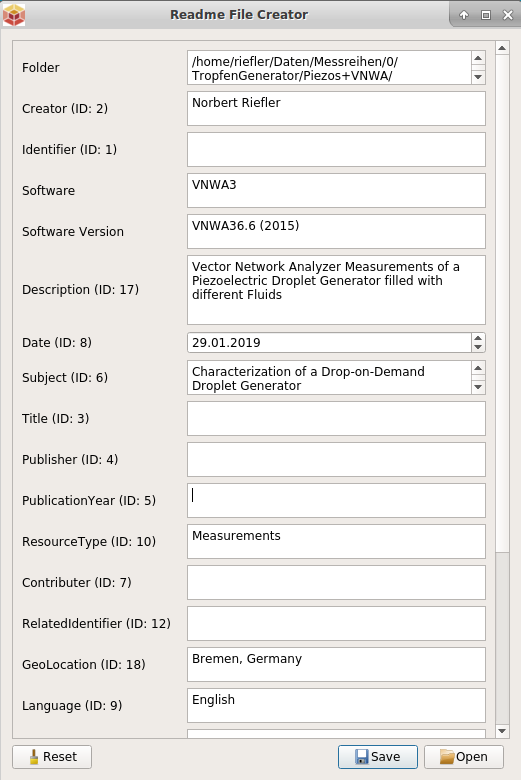
\includegraphics[width=\linewidth]{Figure02_ReadmeFileCreator.png}
  \caption{Data Input Tool: Readme-File-Creator}
  \label{fig:readme-creator}
\end{wrapfigure}
Im Folgenden werden einige der extrahierten Eigenschaften erläutert; weitere
Informationen finden Sie in Tabelle 3 in \cite{datacite2019}: \\[6pt]
%
\textbf{ID 1: Kennung} \\
Nummer, die zur Identifizierung der Daten verwendet wird. Dies kann ein DOI
(Digital Object Identifier) im Falle einer Veröffentlichung oder eine PID
(Persistent Identifier) aus dem ELN sein (eLabFTW  generiert eine lange Nummer
für jedes Experiment, siehe \ref{ssc:ELN} \nameref{ssc:ELN}). \\[6pt]
%
\textbf{ID 2: Erstellerin oder Ersteller} \\
Name der Person, die für die beschriebenen Daten verantwortlich ist (ORCID, Open Researcher Contributor Identification). \\[6pt]
%
\textbf{ID 3: Titel} \\
Kann der Titel eines Datensatzes, der Name einer Software oder der Titel eines
Artikels sein. \\[6pt]
%
\textbf{ID 4: Herausgeber} \\
Der Name der Einrichtung, die die Daten produziert, aufbewahrt, archiviert,
veröffentlicht, druckt, vertreibt, freigibt oder herausgibt (z.B.
"Leibniz-Institut für Werkstofforientierte Technologien - IWT"). \\[6pt]
%
\textbf{ID 5: Jahr der Veröffentlichung} \\
Das Jahr, in dem die Daten öffentlich zugänglich gemacht wurden oder werden. \\[6pt]
%
\textbf{ID 8: Datum} \\
Entstehungsdatum der Daten, einschließlich des Start- und Enddatums des
Projekts, des Datums der Datenänderung und des von den Daten abgedeckten. \\[6pt]
%
\textbf{ID 9: Sprache} \\
Sprache(n) des Inhalts der Quelle. \\[6pt]
%
\textbf{ID 10: Ressourcentyp} \\
Eine Beschreibung der Ressource; meist "DataSet", kann aber auch "\verb+Audiovisuell+",
"High-Speed Images", "DataPaper", etc. sein.\\[6pt]
%
\textbf{ID 19: Förderkennzeichen} \\
Organisationen oder Behörden, die die Forschung finanziert haben. \\[6pt]
%
\textbf{ID 16: Rechte} \\
Alle bekannten Rechte am geistigen Eigentum an den Daten. Die beste Wahl ist
normalerweise die Creative Commons Lizenz 'CC-BY' (BY attribution) oder 'CC-0'
für Daten sowie die 'CC Version 4.0' für schriftliche Dokumente. \\[6pt]
%
\textbf{ID 17: Beschreibung} \\
Wie die Daten erzeugt wurden, einschließlich der verwendeten Geräte oder
Software, des Versuchs\-protokolls und anderer Dinge, die Sie in ein Laborjournal
aufnehmen könnten. \\[6pt]
%
\textbf{ID 18: Geolokalisierung} \\
Wenn sich die Daten auf einen physischen Ort beziehen, halten Sie Informationen
über die geografische Abdeckung fest. \\[6pt]
%
Das oben in \autoref{fig:readme-creator} abgebildete Tool kann vom IWT-File-Server ($\rightarrow$Austausch $\rightarrow$Forschungs\-datenmanagement $\rightarrow$DataManagementGuidelines-ServiceFiles $\rightarrow$ReadmeFileCreator) für jedes Betriebssystem  heruntergeladen werden, um die Eingabe von Metadaten zu vereinfachen. Sie  können automatisch eine Datei namens 'readme.json' mit Ihren Metadaten, eingebettet in ein JSON (Java Scipt Object Notation)-Format, erstellen, die sowohl als Dokumentation als auch als Metadaten für Data Science Methods verwendet wird. Diese Datei wird in jedem Verzeichnis gespeichert, das Daten oder Programmcode enthält. Felder können einfach leer bleiben, wenn sie unzutreffend sind.\\
%
Dieselbe DataCite-Metadaten-Struktur kann auch im JSON-Editor des ELNs (siehe Kapitel \ref{ssc:ELN}) abgebildet bzw. eingegeben werden.


\subsection{Erzeugen eines Metadaten-Schema}
Ein Schema ist eine logische Struktur, die sowohl die Beziehungen zwischen den Metadaten-Elementen aufzeigt als auch Regeln für die Anwendung und Verwaltung der Metadaten liefert. Ein Beispiel für die Entwicklung eines Metadaten-Schema ist in der Arbeit von Eberskirch et al. \cite{elberskirch:2022} beschrieben, in der alle relevanten Parametern gesammelt wurden zur physikalischen als auch biologischen (toxikologischen) Charakterisierung von Nanopartikeln.
Die Entwicklung eines für die eigene Fachdisziplin passenden Schemas kann sehr hilfreich sein für die Strukturierung der Daten und des eigenen Wissens.







\section[Electronic Lab Notebooks]{Electronic Lab Notebooks (ELNs)}\label{ssc:ELN}

Electronic Lab Notebooks (ELNs) enable researchers to organize and store
experimental procedures, protocols, notes and data using their computer or
mobile device. ELNs can offer several advantages over the traditional paper
notebook in documenting research during the active phase of a project, including
searchability within and across notebooks, secure storage with multiple
redundancies, remote access to notebooks, and the ability to easily share
notebooks among team members and collaborators.

\subsection{eLabFTW}

This is an OpenSource, generic, browser based ELN, developed/initialized by
Nicolas Carpi (Institut Pasteuer, Paris) 2012. Data are stored in MySQL/MariaDB.
It is maintained by many developers and is used worldwide (Berkley, Indian
Institute of Technology, KIT, ...).
\begin{itemize}
  \item Access: \url{https://eln.mvt-bremen.de/} or \url{https://134.102.38.139}
  \item Free definable status of the experiments (“finished”, “running”, ...)
  \item Definition of templates for a step-by-step procedure description of
        measurements
  \item Every experiment gets a unique ID and can be summarized easily as a pdf
  \item Free definable categories/tags
  \item Graphical text editor to describe your experiments and simulations
  \item File attachments of data with preview of common formats (pdf, tiff, png, …)
  \item linking of experiments
  \item Time stamp service (RFC 3161, e.g. DFN)
  \item Data import/export (csv, zip, json, …)
  \item access using, e.g., Python via an Application Programming Interface (API)
\end{itemize}

You have to create a pdf for every experiment simply by a click (‘Make a pdf’)
in the edit mode (see \texttt{‘04\_PrimaryData’} in Table
\ref{table:paper-directory-structure}. This kind of documentation includes a
unique QR-code and is required for data which is published! The QR-code enables
a direct link to the data together with unique ID.

The \textbf{maximum size} of uploaded data should not exceed
\textbf{100Mbyte per file}. Further hints and tricks may be found in the seafile
document (please add comments there if you explore new ways of usage): \\
\url{https://seafile.zfn.uni-bremen.de/f/fe685882eab14a2e853c/}

\section{Git}

Git ist ein webbasiertes Tool, das ein Repository für die Versionskontrolle
bereitstellt. Es wird verwendet, um Ihre Softwareentwicklungen zu verwalten, zu
planen, zu erstellen, zu verifizieren und zu überwachen. Außerdem kann es als
System zur Versionierung von Dokumenten verwendet werden. Bei der Erstellung
eines größeren Textes (Dissertation, Referate, Anträge, ...) kann zum
Beispiel der aktuellen Stand des Dokuments eingeben werden, und alle vorherigen
Versionen werden mitgespeichert. Damit lässt sich jeder geänderte Satz
nachvollziehen und rekonstruieren.\\
Wir haben derzeit zwei Git-Instanzen am IWT:
\begin{itemize}
  \item Ein GitLab als Teil des VT-Servers für nicht-öffentliche Dokumente
        \begin{itemize}
          \item[$\rightarrow$] Anmeldung bei den Administratoren siehe in \nameref{ssc:Dateiorganisation} \ref{ssc:Dateiorganisation}
        \end{itemize}
  \item Öffentliches Git: \url{https://github.com/Leibniz-IWT/}
        \begin{itemize}
          \item[$\rightarrow$] Anmeldung: Email mit dem Betreff “IWT Organization access
                               request” an: 
                               \href{mailto:github@iwt.uni-bremen.de}%
                               {github@iwt.uni-bremen.de}
        \end{itemize}
\end{itemize}

\section{EndNote}

We have EndNote as literature management software for everyone (single user
system). EndNote can be integrated into Word to manage cited references in
publications. It also serves as a literature database for papers, textbooks,
presentations etc. And it is used as the literature database for all
publications from the IWT.

\section{Further Tools for Data Management}

\begin{itemize}
  \item Search for Data Repositories: \url{https://www.re3data.org/}
  \item \url{https://zenodo.org/}  $\rightarrow$ scientific data, publications,
        reports, presentations, videos, etc.
  \item \url{https://www.ukdataservice.ac.uk/manage-data/format/recommended-formats}
        \begin{itemize}
          \item[$\rightarrow$] list of recommended data formats
        \end{itemize}
  \item \url{http://rd-alliance.github.io/metadata-directory/standards/}
        $\rightarrow$ Metadata Discipline Standard Formats
  \item Renaming Tools: PSRenamer, ExifToolGUI
\end{itemize}


\appendix
\addcontentsline{toc}{section}{Bibliography}
\printbibliography
\pagebreak
\section{Appendix}
\subsection{How to Store Papers – `Dummy Paper'}\label{app:dummy-paper}
\begin{wrapfigure}{r}{0.5\linewidth}
  \vspace{-1em}
  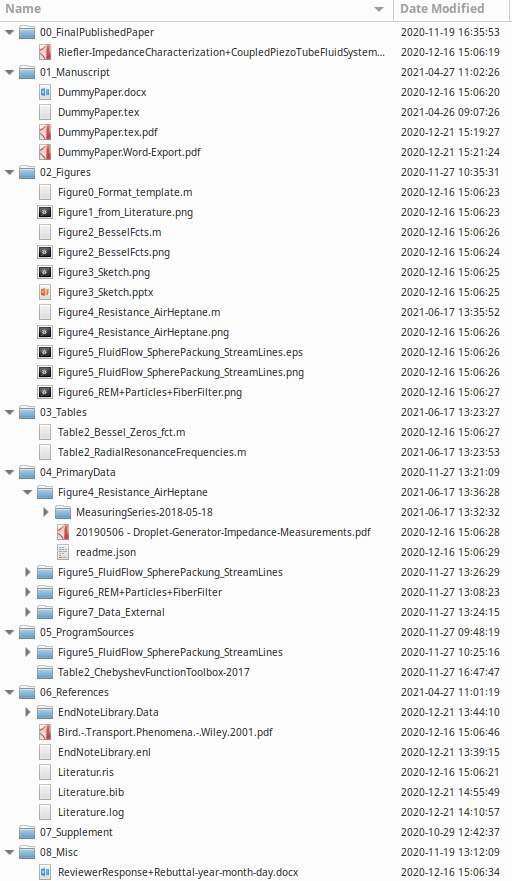
\includegraphics[width=\linewidth]{Figure03_DummyPaperStructureExample4.png}
  \caption{Complete data structure of a dummy paper.}
  \label{fig:dummy-paper}
\end{wrapfigure}
The following screenshot shows a complete data structure of a dummy paper.
You may find this dummy paper on our IWT file server under $\rightarrow$Austausch $\rightarrow$For\-schungsdatenmanagement $\rightarrow$Data\-Manage\-mentGuidelines-ServiceFiles  $\rightarrow$DummyPaper. Basically, the idea is that every data in the
paper, whether it is a figure or a table, can be related to the original source
of the measurement or the simulation. This is realized in the Dummy Paper by
Matlab scripts, but can be done using other means as well (Python, Excel). The
point is: No matter how, but you have to give a relation between the data saved
in the \texttt{‘04\_PrimaryData’} directory and their representation in the
publication. All figures and their generating scripts – here Matlab files – are
given together with the measurement data so that running a Matlab (Octave)
script within that directory generates the according figure. In the end, someone
else can reproduce your results given in your publication. In case of other data
like SEM images for instance, you can refer to them by a PDF generated by the
ELN including a link to the experiment stored there.

The `Dummy Paper' contains a Word and a LaTeX template in
\texttt{‘01\_Manuscript’}. The EndNote or BibTeX literature references are in
\texttt{‘06\_References’}. Both, the EndNote file ‘*.enl’ or the BibTeX file
‘*.bib’, should include links between the references and the freely accessible
PDFs of the papers and books also saved in \texttt{‘06\_References’}.

\subsection{How to Write a DMP}

\subsubsection{Motivation}

A Data Management Plan (DMP) documents the thoughts of an applicant about the
data which will be generated during the applied research project. Research
funders (DFG etc.) expects that publicly promoted projects makes their data
accessible to the public, where a simple publication was sufficient in the past.

There is no unified structure of DMPs due to the vast number of different
research tasks. In the following, the main elements of a DMP from the
TIB Hannover are listed, which can be found also in the recommendation of the
DFG: \\
(\url{https://www.dfg.de/download/pdf/foerderung/grundlagen_dfg_foerderung/forschungsdaten/forschungsdaten_checkliste_de.pdf})

\subsubsection{Elements of a DMP}

\begin{enumerate}[start=0, label=\textbf{\arabic*})]
  \item \textbf{Administrative information}
        \begin{itemize}
          \item Project name
          \item Project participants
          \item Project description
          \item Project ground (doctorate, third party funding, etc.)
          \item Project duration
          \item Version of this DMP
        \end{itemize}
  \item \textbf{Methods and kinds of data gathering}
        \begin{itemize}
          \item Are there primary data generated, or will be secondary data used?
          \item Which data types / formats are generated and processed?
          \item How large are the data?
          \item Which equipment (instruments, hardware, software, etc.)
                will be used?
          \item How are the data organized? (Directory of file oriented
                structure? Version control?)
          \item How is the research process and the data been documented?
          \item Which (technical) standards will be used for
                description/documentation (metadata, classification)?
          \item How are the metadata been generated (e.g. automatically,
                manually, after a guideline, self-defined)?
        \end{itemize}
  \item \textbf{Backup and data safety}
        \begin{itemize}
          \item Where are the data stored?
          \item Which capacity is required?
          \item Interval of data safety?
          \item Are there any protective measures required for sensitive data?
          \item Are there any third party of project partners (e.g. in joint
                projects) who need access to the data?
        \end{itemize}
  \item \textbf{Archiving}
        \begin{itemize}
          \item Which data is archived?
          \item On which data carrier?
          \item Are there any requirements for the operators of the
                infrastructure? E.g. data curation?
          \item Which metadata have to be provided to find the archived data?
          \item Which information is additionally required to understand the
                context of the data?
          \item How long are the data archived?
          \item Are there any legal technicalities for the data archiving?
          \item What are the costs for which service?
        \end{itemize}
  \item \textbf{Data sharing and publication}
        \begin{itemize}
          \item Are there data which must be shared with others?
          \item What are the possible systems for data sharing?
          \item Which metadata and documentation are additionally required for
                third parties to use the data?
          \item Where (data repository, data journal) will the data be
                published, and how (e.g. open access, with embargo time,
                restricted access)?
          \item What are the license condition for the published data?
                (E.g. `CC BY 4.0')
        \end{itemize}
  \item \textbf{Resources and responsibilities}
        \begin{itemize}
          \item How is the distribution of responsibility governed in this project?
          \item How is responsible for the data management (processes, IT,
                guidelines, formats, monitoring)?
          \item Required personal resources for a successful
                implementation/realization?
          \item What are the costs within the project phase and
                possibly thereafter?
          \item Which infrastructure resources are required, with additionally
                costs?
        \end{itemize}
\end{enumerate}




\pagebreak
\subsection{Glossary}

\begin{table}[h]
\begin{tabular}{lll}
AiF   & $\ldots$  & Arbeits�gemeinschaft industrieller Forschungs�vereinigungen \\
ASCII & $\ldots$  & American Standard Code for Information Interchange \\
BMBF  & $\ldots$  & Bundesministerium f�r Bildung und Forschung \\
BSD   & $\ldots$  & Berkeley Software Distribution \\
CC-BY & $\ldots$  & Creative Commons - BY attribution \\
DFG   & $\ldots$  & Deutsche Forschungs-Gemeinschaft \\
DMP   & $\ldots$  & Data Management Plan \\
ELN   & $\ldots$  & Elektronic Laboratory Notebook \\
ERC   & $\ldots$  & European Research Council \\
FAIR  & $\ldots$  & Findable Accessible Interoperable Reusable \\
GWP   & $\ldots$  & Gute Wissenschaftliche Praxis \\
ISO   & $\ldots$  & International Organization for Standardization  \\
JSON  & $\ldots$  & Java Script Object Notifier \\
NAS   & $\ldots$  & Network Access Storage \\
XML   & $\ldots$  & eXtended Markup Language \\

\end{tabular} {lll}
\end{table}




\end{document}
